\section{Szegedy quantum walk}

The following method proposed by Szegedy helps to reduce some limitations discussed in the previous section. In order to 
talk about this method we need to introduct some concepts.

\subsection{Markow chains}

A Markow chain is a stochastic process that consists in a sequence of random variables $X_{n}$ with $n \in \mathbb{Z}^{+}$
such that:

\begin{equation}
    \scriptstyle P(X_{n} | X_{n-1}, X_{n-2},...,X_{n-N}) = P(X_{n} | X_{n-1})
\end{equation}

If is time-independent can be represented by a matrix P called transition matrix. Such that the sum of each row of P is equal to 1.

\subsection{application to graphs}

We can use then a Markow Chain to represent the graph. First, considering a graph G(V,E) we construct the adjacency matrix
as follows:

\begin{equation}
    A_{i,j} = 
    \begin{cases} 
        1\, if (v_{i}, v_{j}) \in E \\
        0\, otherwise
    \end{cases}
\end{equation}

Then we can define the transition matrix P as $P_{i,j} = \frac{A_{i,j}}{indeg(j)}$ where indeg(j) 
represents the number of in-going edges of vertex j. In the 
cyclic graph $C_{8}$ (Fig. 6a) each node has 2 in-going edges therefore the transition matrix is:

\begin{equation*}
    P = \frac{1}{2}
    \begin{pmatrix}
    0 & 1 & 0 & 0 & 0 & 0 & 0 & 1 \\
    0 & 0 & 1 & 0 & 0 & 0 & 1 & 0 \\
    0 & 1 & 0 & 1 & 0 & 0 & 0 & 0 \\
    0 & 0 & 1 & 0 & 1 & 0 & 0 & 0 \\
    0 & 0 & 0 & 1 & 0 & 1 & 0 & 0 \\
    0 & 0 & 0 & 0 & 1 & 0 & 1 & 0 \\
    0 & 0 & 0 & 0 & 0 & 1 & 0 & 1 \\
    1 & 0 & 0 & 0 & 0 & 0 & 1 & 0 \\
    \end{pmatrix}
\end{equation*}

Express the graph with this transition matrix give us more flexibility, the previous 
method used directly labels encoding and was limited to undirected graphs without weights. The Szegedy algorithm works by quantizing the markow chain, here there are no problem if the graph is directed
or has weights. 

\subsection{The szegedy QW operator}
The szegedy quantum operator seems quite similar in aspect to coined quantum walk operator but there are lot of differences in the behavior. 
The space we consider now is an Hilbert space composed by 

\begin{equation}
    \mathcal{H} = \mathcal{H}_{1}^{N} \otimes \mathcal{H}_{2}^{N}
\end{equation}

where N is the number of graph's nodes and $\mathcal{H}$ has dimension $N^2$. To understand why we can anticipate that this operator works in the bipartite graph genereted copying the original node set. 
We construct 2 sets, X and Y each containing the nodes of the original graph, the bipartite graph will be 
made by connect nodes between X and Y if they are adjacent, the Fig. 6b below will hopefully clarify this concept, it shows the bipartite graph associated
to the cycli graph $C_{8}$ showed in Fig. 6a.


\begin{figure}[h!]
    \centering   
    \subfigure[Figure A]{\label{fig:a}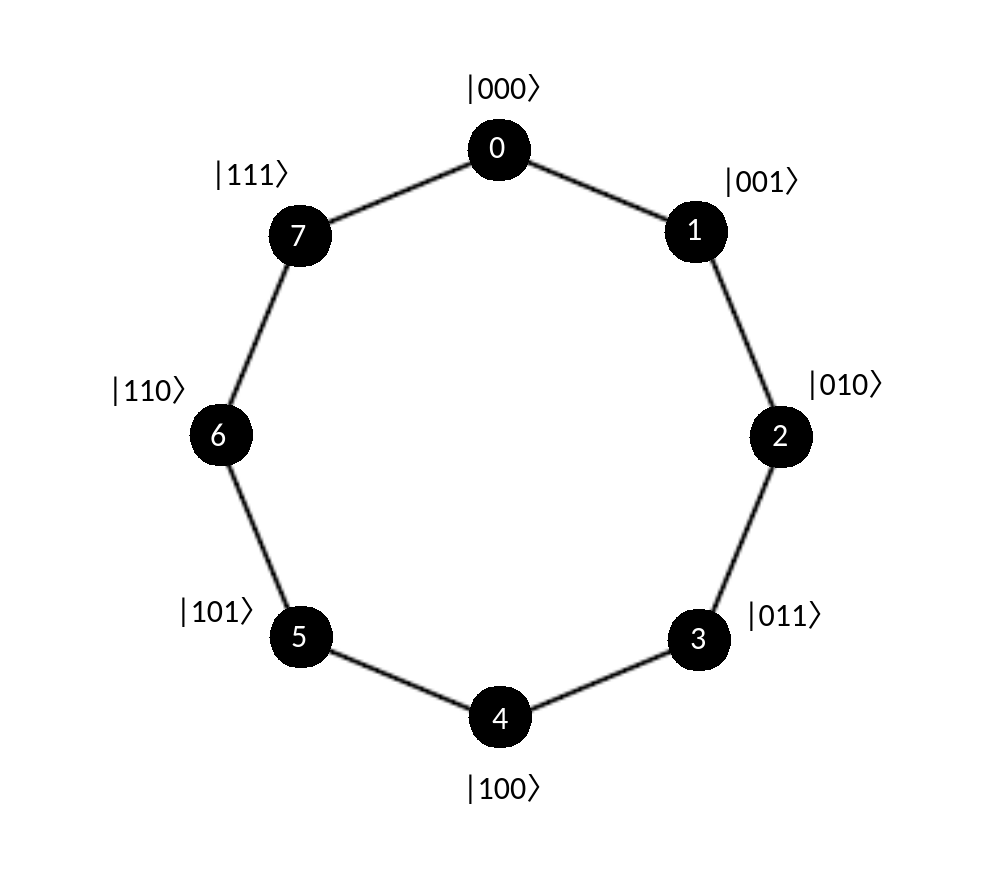
\includegraphics[scale=0.3]{img/cyclic_graph.png}}
    \subfigure[Figure B]{\label{fig:b}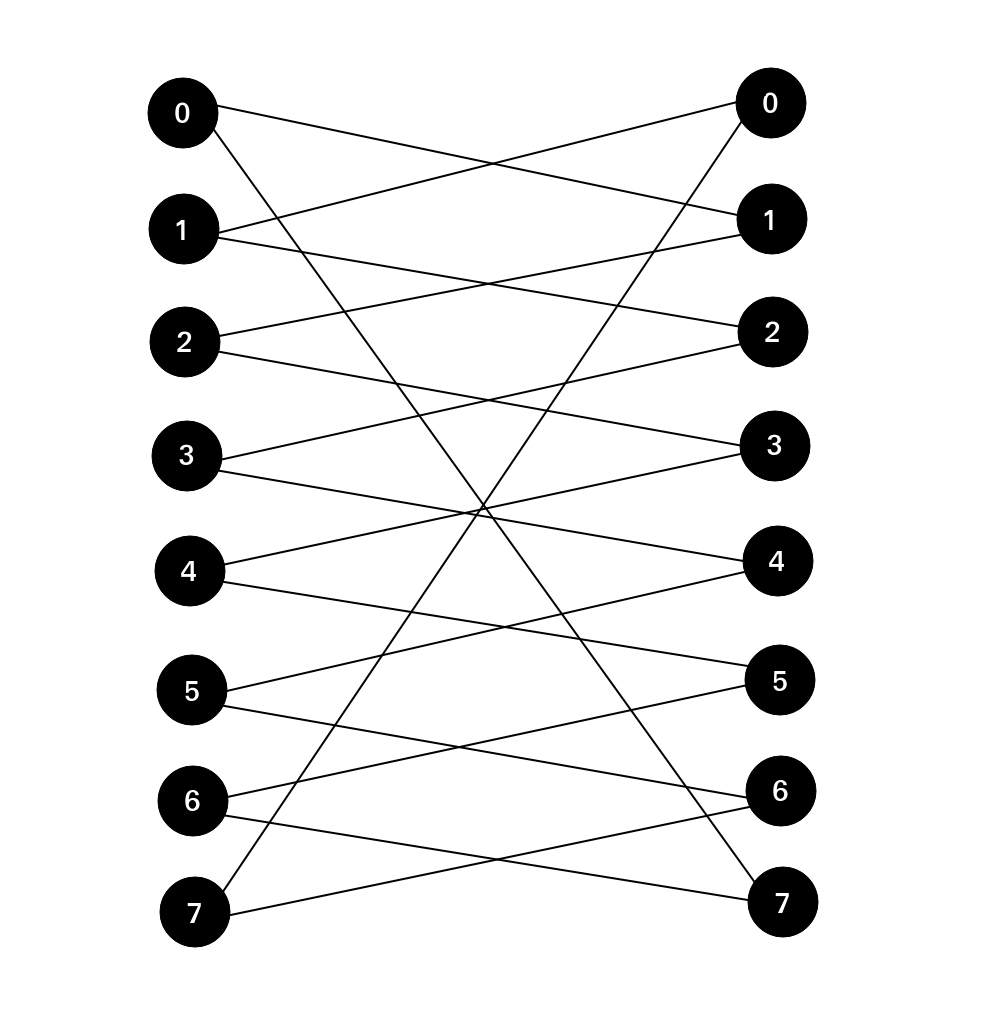
\includegraphics[scale=0.3]{img/bipartite.png}}
    \caption{Fig. A shows the cyclic graph, already used for the coined QW, Fig. B shows the correspondent bipartite graph constructed using the sets X and Y which contains the nodes of the cyclic graph
    edges connect only adjacent nodes of the cyclic graph.}
\end{figure}

Before introducing the Szegedy operator we need to define some operators that compose it, like in the coined quantum walk where the 
walk operator was composed by the coin and position operator here we have two different operators called Reflection Operator (R) and Swap Operator (S). To introduce
the R operator we need the state vector that represent the system, is given by $\ket{\psi} \in \mathcal{H}$ and is equal to:

\begin{equation}
    \ket{\psi} = \sum_{i=0}^{N-1}\sum_{j=0}^{N-1} a_{i,j}\ket{i,j} 
\end{equation}

Then we define the projector states of the markow chain:

\begin{equation}
    \ket{\psi_{i}} = \ket{i} \otimes \sum_{j=0}^{N-1}\sqrt{P_{j+1,i+1}}\ket{j} \equiv \ket{i} \otimes \ket{\phi_{i}}
\end{equation}

where $\ket{\phi_{i}}$ is the square-root of the \textit{i}-th column of the transition matrix P. The projector operator Then is given by:

\begin{equation}
    \Pi = \sum_{i=0}^{N-1}\ket{\psi{i}}\bra{\psi{i}}
\end{equation}

with the associated Reflection Operator:

\begin{equation}
    \mathcal{R} = 2\Pi - I
\end{equation}

The second operator needed is the Swap operator S given by:

\begin{equation}
    \mathcal{S} = \sum_{i=0}^{N-1}\sum_{j=0}^{N-1} \ket{i,j}\bra{j,i} 
\end{equation}

Finally the one-step Szegedy QW operator is given by:

\begin{equation}
    U_{walk} = S(I - 2\varPi) = SR
\end{equation}

This doesn't want to be a formal explanation, the schematized concepts above came from \cite{Loke_2017} and are just a summary helpful for the implementation. 
The concept behind the operator are covered with more details in \cite{c2dacf48ddf341aca084f825d3787894, Loke_2017,1366222}, 
\cite{Portugal2018} from Pag. 224 and also \cite{Wong2017} (which provides an example for a cyclic graph with 6 nodes), since \cite{c2dacf48ddf341aca084f825d3787894, Loke_2017, 1366222}
were a difficult reading for me this last two more theoretic references helped me understand some concepts and get the basic idea, especially \cite{Wong2017}. 

\section{Szegedy Quantum Walk Implementation}

For the Implementation in qiskit I used as refereces \cite{Loke_2017} and \cite{c2dacf48ddf341aca084f825d3787894}, where I also found the generic circuit 
to implement the szegedy QW on a cyclic graph.

As for the coined quantum walk, the circuit is said to be efficent if the one and two qubits gates used are no more than O(Poly(log(N))) with N number of nodes. 
While for S there are no problems R operator in this
form cannot be implemented efficiently, \cite{Loke_2017} provide a way to implement it efficiently diagonlizing the operator R. Fig. 7 taken from that
paper represent the generic circuit for the Szegedy QW on a $C_{N}$ graph and shows how R is separated in order to realize the circuit efficiently. 


\begin{figure}[h!]
    \centering   
    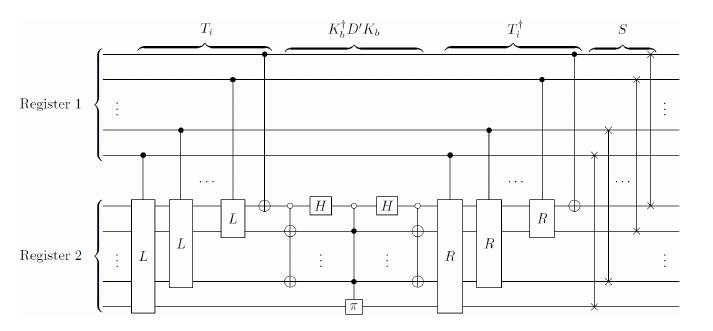
\includegraphics[scale=0.4]{img/generic_szegedy.jpg}
    \caption{Generic Circuit for the Szegedy Quantum Walk on a Cycle graph with N nodes, this image is taken from}
\end{figure}

The L and R subcircuit are called respectively one-element left rotation and one-element right rotation, are used to perform a cyclic permutation
of the vector given as input and are efficiently implementable requiring at most $log(N)$ qubits (a sequence of multi C-NOT). Swap are trivially 
efficiently implementable. In Fig. 8 below there is the specific circuit for the one-step Szegedy Quantum Walks on the cyclic graph $C_{8}$.

\begin{figure}[h!]
    \centering   
    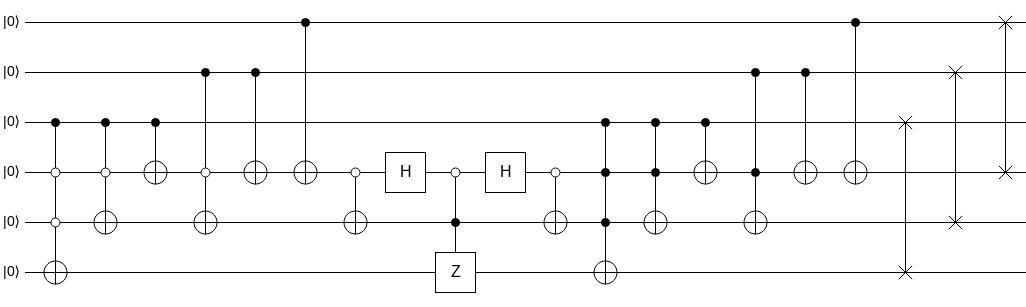
\includegraphics[scale=0.25]{img/szegedy_c8.jpg}
    \caption{Circuit for the Szegedy QW on a cyclic graph}
\end{figure}

To make an example we can prepare the initial state of the walker as a superposition $\ket{psi_{0}} = \ket{0} \otimes \ket{\phi_{0}}$
where $\ket{\phi{0}} = [0, frac{1}{\sqrt{2}}, 0 , 0, 0, 0, 0, frac{1}{\sqrt{2}}]$ and we expect as output in the first register $R_{1}$ an equiprobability of the adjacent nodes.

\href{https://algassert.com/quirk#circuit={%22cols%22:[[1,1,1,%22H%22,1,%22X%22],[1,1,1,%22%E2%80%A2%22,%22X%22],[1,1,1,%22Amps3%22],[],[1,1,1,%22Chance3%22],[1,1,%22%E2%80%A2%22,%22X%22,%22%E2%97%A6%22,%22%E2%97%A6%22],[1,1,%22%E2%80%A2%22,1,%22X%22,%22%E2%97%A6%22],[1,1,%22%E2%80%A2%22,1,1,%22X%22],[1,%22%E2%80%A2%22,1,%22X%22,%22%E2%97%A6%22],[1,%22%E2%80%A2%22,1,1,%22X%22],[%22%E2%80%A2%22,1,1,%22X%22],[1,1,1,%22%E2%97%A6%22,%22X%22],[1,1,1,%22H%22],[1,1,1,%22%E2%97%A6%22,%22%E2%80%A2%22,%22Z%22],[1,1,1,%22H%22],[1,1,1,%22%E2%97%A6%22,%22X%22],[1,1,%22%E2%80%A2%22,%22X%22,%22%E2%80%A2%22,%22%E2%80%A2%22],[1,1,%22%E2%80%A2%22,1,%22X%22,%22%E2%80%A2%22],[1,1,%22%E2%80%A2%22,1,1,%22X%22],[1,%22%E2%80%A2%22,1,%22X%22,%22%E2%80%A2%22],[1,%22%E2%80%A2%22,1,1,%22X%22],[%22%E2%80%A2%22,1,1,%22X%22],[1,1,%22Swap%22,1,1,%22Swap%22],[1,%22Swap%22,1,1,%22Swap%22],[%22Swap%22,1,1,%22Swap%22],[%22Amps3%22],[],[%22Chance3%22,1,1,%22Chance3%22]]}}{Click this simulation in Quirk} 
to see what mentioned above, again in the simulation multi controlled toffoli are specular since Quirk uses the little-endian convention.

\subsection{Comparison with classical}

The measure in which we compare those type of algorithm is in Hitting Time, this value in a stochastic process is the first time 
at which the given process "hits" a given set of substate. The famous paper of Szegedy \cite{1366222} which is the starting point of this
algorithm shows that in a certain condition we can achive a quadratic speed-up. Unfortunataly this paper was too hard for me to understand 
therfore i will not go deeper in this topic. 